\chapter{Chess-game analysis}

\section{The game of chess}

Chess is a two-player turn-based strategy game played on a checkered board with bounded dimensions: 64 squares arranged in an 8×8 grid, where each player has a set of initial pieces arranged in a specific order aiming to conquer an specific opponent piece: The King.

In game-theory, Chess is classified in the cluster of games with perfect information in which the players move alternately and the game is not subject to randomization.

The history of chess was firstly documented around 6th Century, although the earliest origins are ambiguous. It is believed that the game's predecessor was originated in India, from where the game spread to Persia. After the Arabic occupation, the game was spread through the Muslim world and to Southern Europe, where it evolved into the current form in the 15th Century ~\cite{murray1913history}.


    \begin{figure}[H]
        \centering
        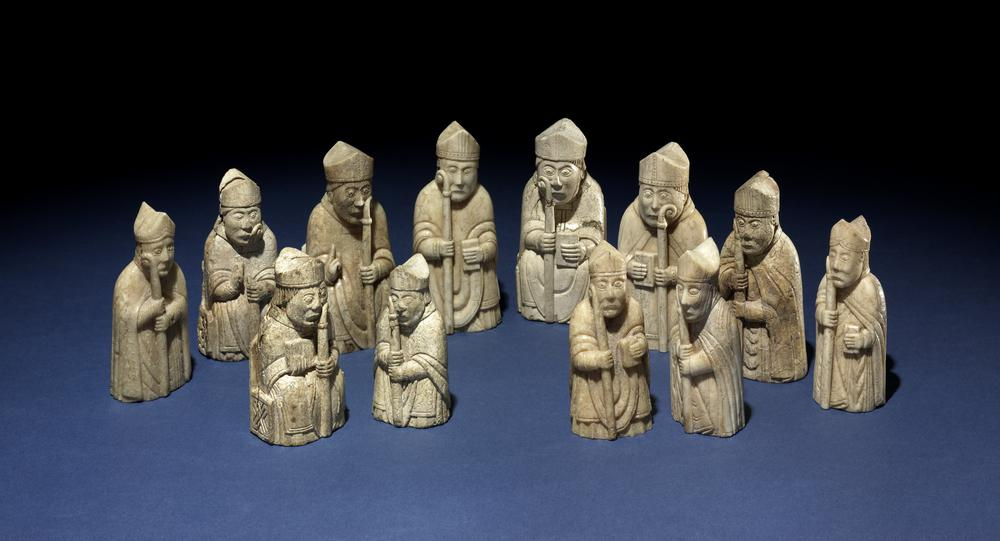
\includegraphics[width=0.6\textwidth]{chessmen}
        \caption{The Lewis chessmen are a group of distinctive 12th-century chess pieces, along with other game pieces, most of which are carved from walrus ivory. Present location: British Museum, London. Image courtesy of Wikipedia Commons}.
    \end{figure}

\section{Computing chess}

\subsection{Zermelo's theorem}

\begin{theorem} 
Zermelo's theorem is a game-theory theorem regarding finite two-person games of perfect information in which the players move alternately and the game is not subject to randomization. It suggests that if the game cannot end in a draw, then one of the two players must have a winning strategy (\textit{i.e. force a win}). 

An alternate statement is that for a game meeting all of these conditions except the condition that a draw is not possible, then either the first-player can force a win, or the second-player can force a win, or both players can force a draw. ~\cite{schwalbe2001zermelo}. 
\end{theorem}

\begin{remark}
As the chess is a finite two-person games of perfect information in which the players move alternately and the game is not subject to randomization, Zermelo's Theorem can be applied for this game. It states that either White can force a win, or Black can force a win, or both sides can force at least a draw.
\end{remark}

With this background of theoretical work, we can state that there must be a perfect algorithm for chess, at least for one of the two players.

\begin{remark}
All endgames of 6 pieces or less have been perfectly solved.
\end{remark}

\begin{remark}
Previous results show that the game of Losing Chess is a win for White. ~\cite{watkins2017losing}. The "losing-winning" move is \textbf{e3} for White.
\end{remark}


\subsection{Chess complexity using Bachmann-Landau notations}

This subsection will present another example of inappropriate use of Bachmann-Landau asymptotic notations for algorithms that do not generalize well. As previously stated, a perfect algorithm for chess exists, even though the state space that it would have to search would be huge. 

Due to finite-bounds of the game and the existence of the 50-move rule, which allows either player to claim a draw if 50 or more moves take place without movement of a pawn  or a piece-capture, based on FIDE-game rules, the longest chess game could be up to 4851 moves. A wide estimation would be counting the total number of possibilities for a the player to move one of (at most) 16 pieces: 8 pawns, each with at most 3 moves, 2 rocks each with at most 14 moves, 2 knights 8 each with at most, 2 bishops, each with at most 14 moves, 28 for a queen and 8 for a king, for a total of 132 possible moves. Definitely these are just hypothetical situation analyzing the worst-case scenario, as in real games the possibilities are far smaller.

Hence, the total number of chess games would be at most $132^{4851}$. (a more realistic estimation would be $10^{500}$)

As a finite game can be simulated in constant time, the above estimation, translated in Bachmann-Landau notations for complexity classes, this means that the perfect algorithm for chess should perform in $O(132^{4851})$. Using the properties of Big-O complexity class, we can state that this algorithm will perform in constant time, with $O(1)$ complexity as this number of total number of chess, regardless how big it is, is still a constant. 

In this situation, the Bachmann-Landau asymptotic notations did not provide useful information and the reason is simple: these notations were developed for asymptotic-scaling problems and algorithms, w/o awareness of discrete values. Even though in most cases these notations were helpful, this is probably not the case in this scenario.

\subsection{Previous work}
Claude Shannon had studied the implications of a brute force solution for solving chess back in the 1950 ~\cite{shannon1950xxii}, when he introduced the \textbf{Shannon number}, a conservative lower bound of the game-tree complexity of chess. The purpose was to validate that any perfect chess algorithms based on brute-force are impractical.

The Shannon number proposed back in 1950 was $10^{120}$, taking into consideration a typical game  of 80 moves at a rate of $10^3$ possibilities for each pair of white-black moves.

Previous work of Claude Shannon was building the foundation of information theory with a landmark paper (1948), \textit{"A Mathematical Theory of Communication"}. 

Further work showed that, based on an average branching factor of 35 and an average game length of 80, the lower bound for the chess game-tree is around $10^{123}$. Victor Allis: ~\cite{allis1994searching}

\section{Chess in r-Complexity}
TODO